\documentclass[
	% handout
]{beamer}
\setbeamertemplate{navigation symbols}{}
\usepackage{xcolor}
\definecolor{seeblau}{HTML}{00A9E0}
\definecolor{seegrau}{HTML}{9AA0A7}

\definecolor{seeblau1}{HTML}{CCEEF9}
\definecolor{seeblau2}{HTML}{A6E1F4}
\definecolor{seeblau3}{HTML}{59C7EB}
\definecolor{seeblau4}{HTML}{00A9E0}
\definecolor{seeblau5}{HTML}{008ECE}

\setbeamercolor{title}{fg=seeblau}
\setbeamercolor{frametitle}{fg=seeblau}
\setbeamercolor{section in toc}{fg=seeblau}
\setbeamercolor{structure}{fg=seeblau}

\setbeamertemplate{footline}{%
	\begin{beamercolorbox}[sep=1em,wd=\paperwidth,leftskip=0.5cm,rightskip=0.5cm]{footlinecolor}
		\small\textbf{\insertsection}\quad\insertsubsection\hfill\insertframenumber
	\end{beamercolorbox}%
}

\usepackage[english]{babel}
\parskip=20pt

\usepackage[sfdefault]{roboto}
\usepackage{sfmath}

\usepackage{ifthen, adjustbox}
\newcommand{\markieren}[4]{
	\ifthenelse{\equal{#1}{}}{}{\adjustbox{padding=3pt, bgcolor=seeblau1, margin=-1pt}{\strut{\sffamily\robotoMedium{#1}}}\\}
  \ifthenelse{\equal{#2}{}}{}{\adjustbox{padding=3pt, bgcolor=seeblau2, margin=-1pt}{\strut{\sffamily\robotoMedium{#2}}}\\}
	\ifthenelse{\equal{#3}{}}{}{\adjustbox{padding=3pt, bgcolor=seeblau3, margin=-1pt}{\strut{\sffamily\robotoMedium{#3}}}\\}
	\ifthenelse{\equal{#4}{}}{}{\adjustbox{padding=3pt, bgcolor=seeblau4, margin=-1pt}{\strut{\sffamily\robotoMedium{#4}}}}
}

\usepackage[
	style=authortitle
]{biblatex}
\newcommand{\customcite}[1]{
\let\thefootnote\relax\footnotetext{
	\tiny\raggedleft
	\emph{\citetitle{#1}}, \citeauthor*{#1} \citeyear{#1}
}
}


\usepackage[ddmmyyyy]{datetime}
\renewcommand{\dateseparator}{.}

\usepackage{amsmath,amssymb,amsfonts,amsthm}

\addbibresource{literature.bib} 
\DeclareMathOperator{\Tr}{Tr}

\author{Leon Oleschko}
\institute{Universität Konstanz}
\date{\today}

\begin{document}
{
\setbeamertemplate{footline}{} 
\begin{frame}
	\huge
	\markieren{}{}{Quantum Measurement}{Zeno Effect}
	
	\vfill
	\normalsize
	Leon Oleschko\\
	\today
	
	\vfill
	\raggedleft
	\small
	\textit{Modeling Quantum Hardware: open dynamics and control}\\
	Universität Konstanz
\end{frame}
}

\begin{frame}{}
	\Large
	No phenomenon is a real phenomenon until it is an observed phenomenon.\\
	\normalsize\raggedleft
	 -- John Archibald Wheeler 1970

	\note{
		In this course, we primarily examined nonlinear phenomena through numerical simulations. Toward the end, we introduced a quantum harmonic oscillator model interacting with a thermal bath.

		Why highlight measurement now?

		Measurement is the bridge between our theoretical models (classical or quantum) and what we actually observe in experiments.
		Wheeler’s insight underscores how observation (or readout) transforms a theoretical prediction into a real outcome.
		
		Especially critical in quantum mechanics, where the act of measuring plays a unique role in determining the system’s state.
	}
\end{frame}

\begin{frame}{Historical Note}
	\begin{itemize}[<+->]
		\item[1900] Plank \& Einstein: Blackbody Radiation
		\item[1920] Bohr, Heisenberg: Copenhagen interpretation\\
								Born: Probabilistic interpretation $P(m) = |\langle m| \psi \rangle|^2$
		\item[1930] EPR Paradox
		\item[1926] Schrödinger: Measurement Problem 
		\item[1932] von Neumann: \textit{Mathematical Foundations of Quantum Mechanics}
		\item[\textcolor{seegrau}{1970}] \textcolor{seegrau}{Decoherence Theory}
		\item[] Experimental Interest
	\end{itemize}
	\note{
		In the 1920s, Bohr and Heisenberg laid the foundation of quantum measurement theory. Today, we harness these principles to build quantum processors. For instance, IBM’s superconducting qubits rely on microwave resonator readouts—just as von Neumann’s postulate suggests.
		Now let’s revisit the formal definition of projective measurements—because these are exactly what’s implemented (at least in an approximate sense) on hardware.
	}
\end{frame}


\section{Strong Measurement}
\begin{frame}{Projective Measurement}
	Measurement Operator $\hat M = \sum m |m\rangle$ on $\psi$:
	$$p(m) = |\langle m|\psi\rangle|^2$$
	$$\psi \xrightarrow{\text{Measuring }m} |m\rangle$$

	{\small\textcolor{seegrau}{
		Neglegting Normalization and Degenercy:
		POVM Measurement
	}}

	\customcite[2.2.3]{nielsen_quantum_2010}
\end{frame}

\begin{frame}{Qubit Example}
	\begin{columns}
		\column{.5\textwidth}
		\begin{align*}
			H &= \sigma_z\\
			|\psi> &\propto |\uparrow\rangle + |\downarrow\rangle
		\end{align*}
		$\Rightarrow$ Superposition is stable

		\only<2>{
			$$M = \sigma_z$$
			$\Rightarrow$ $p(\uparrow) = p(\downarrow)$
		}


		\column{.5\textwidth}
		\centering
		\only<1>{
			\includegraphics{figures/03 free.pdf}
		}
		\only<2>{
			\includegraphics{figures/03 measurement.pdf}
		}
	\end{columns}
\end{frame}

\begin{frame}{Decay}
	
\end{frame}



\begin{frame}{Discrete Zeno}
	\begin{center}
		\includegraphics{figures/04 discreate zeno.pdf}
	\end{center}
\end{frame}


\section{Weak Measurement}
\begin{frame}{Weak Measurement}
	\begin{center}
		\includegraphics[width=\textwidth]{figures/Fig. 8.4.jpg}
	\end{center}
	\customcite[]{vladimir_braginsky_quantum_1992}
\end{frame}

\begin{frame}{Rabi Oscillations Setup}
	\begin{columns}
		\column{.5\textwidth}
		\begin{center}
			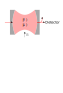
\includegraphics{figures/rabi.pdf}
		\end{center}

		\column{.5\textwidth}
		\begin{align*}
			H &= g\; (a^\dagger a) (\sigma^+ \sigma^-) &\text{Coupling}\\
			&+ g_s\; (\sigma^+ + \sigma^-) &\text{Magnetic}\\
			&- i \beta (a^\dagger - a) &\text{Optic}\\
			J &= \kappa\; a &\text{Dissipation}\\
			C &= \sqrt{\kappa\eta}\; a &\text{Measurement}
		\end{align*}
		
	\end{columns}

	\customcite{nielsen_stochastic_2008}
\end{frame}

\begin{frame}{Time evolution}
	\includegraphics{figures/02 rabi w measurement.pdf}
\end{frame}


{
	\setbeamercolor{background canvas}{bg=black}
	\begin{frame}[plain]{}\end{frame}
}

\section{Appendix}
% \input{notes_sql.tex}

\end{document}